\makesection{Rendering}

\begin{frame}{Rendering Architecture}
    \centering
    % Define the style for the boxes
    \begin{tikzpicture}
        % Main Renderer
        \node[draw, thick, minimum width=10cm, minimum height=2cm] (main) {Main Renderer};

        % Subrenderers: TerrainRenderer, HUDRenderer, EntityRenderer
        \node[draw, thick, minimum width=3cm, minimum height=1cm, below=1cm of main, xshift=-3.5cm] (entity) {Entity Renderer};
        \node[draw, thick, minimum width=3cm, minimum height=1cm, below=1cm of main] (hud) {HUD Renderer};
        \node[draw, thick, minimum width=3cm, minimum height=1cm, below=1cm of main, xshift=3.5cm] (terrain) {Terrain Renderer};

        % Arrows from main renderer to subrenderers
        \draw[->, thick] (main.south) -- (entity.north);
        \draw[->, thick] (main.south) -- (terrain.north);
        \draw[->, thick] (main.south) -- (hud.north);
    \end{tikzpicture}
\end{frame}

\begin{frame}{Rendering Architecture}
    \begin{tabular}{ccc}

        \parbox{0.3\textwidth}{
            \centering \textbf{Entity Renderer}
            \vspace{0.2cm}
            \begin{itemize}
                \item Entities are rendered with their respective textures
                \item Handles animations of the entities, e.g. walking
            \end{itemize}
            \vspace{0.5cm}
            \centering
            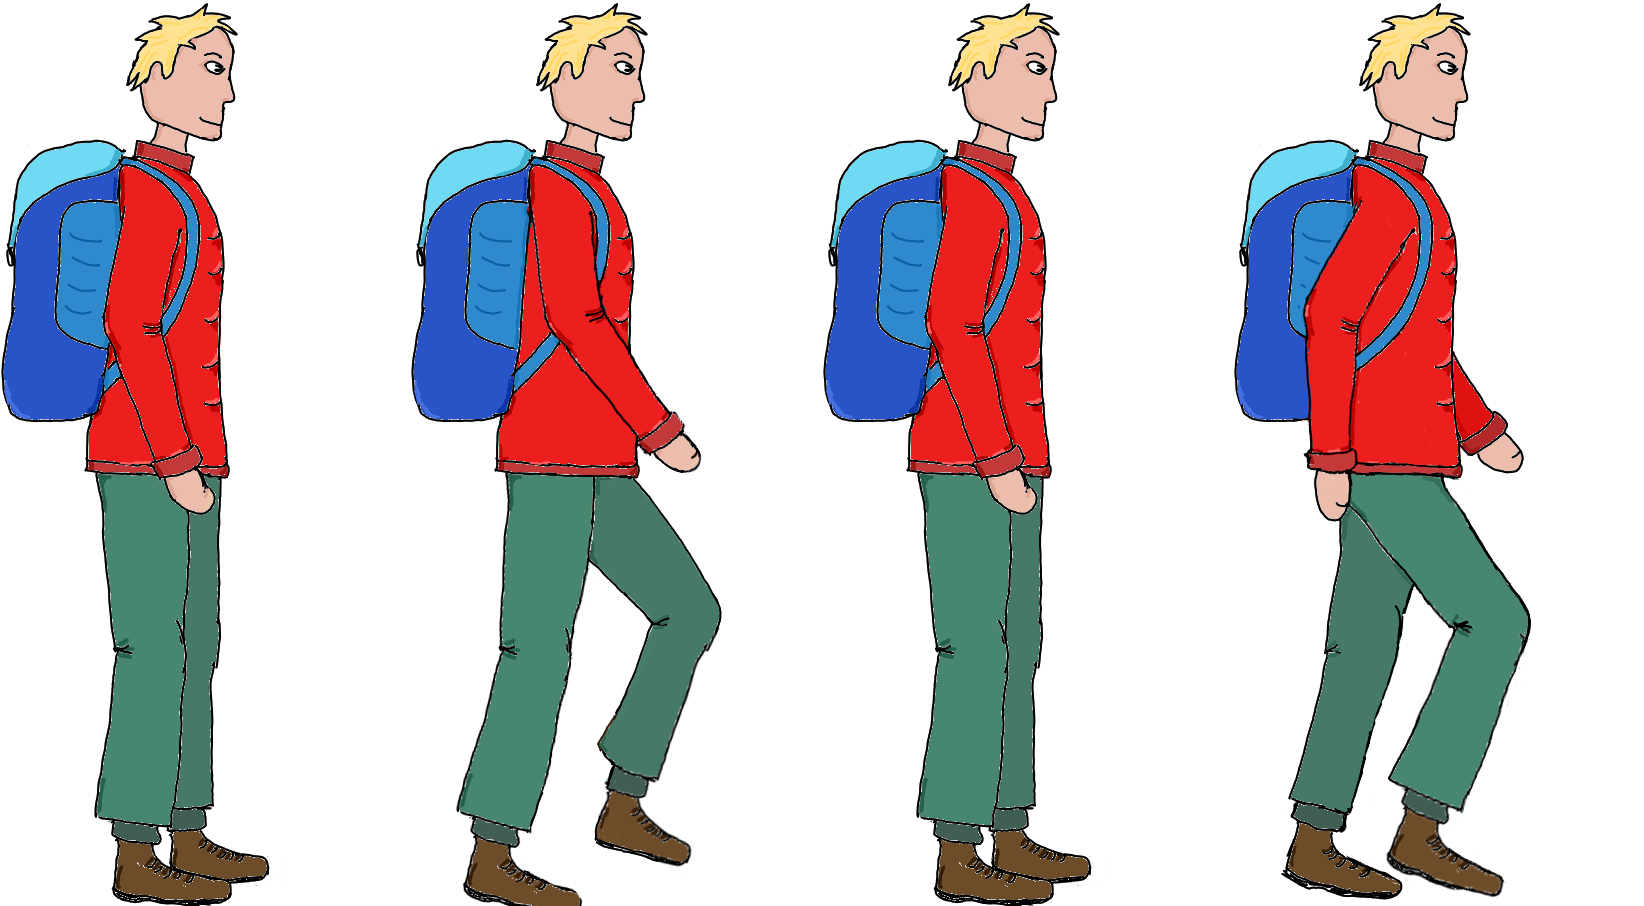
\includegraphics[width=0.25\textwidth]{../../assets/texture/player_walk.png}
        } &

        \pause
        
        \parbox{0.3\textwidth}{
            \centering \textbf{Terrain Renderer}
            \vspace{0.2cm}
            \begin{itemize}
                \item Terrain is continuously rendered with a texture
            \end{itemize}
            \vspace{0.5cm}
            \centering
            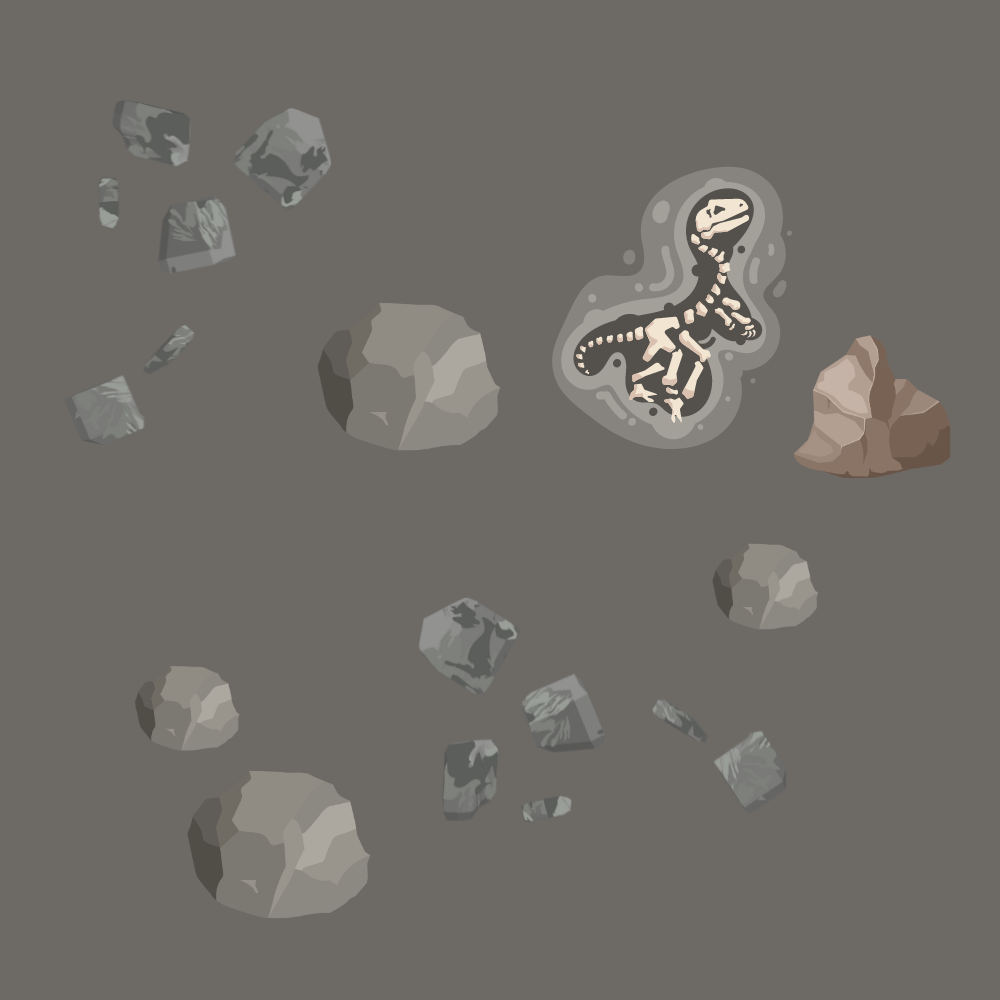
\includegraphics[width=0.2\textwidth]{../../assets/layers/mountain3.png}
        } &

        \pause
        
        \parbox{0.3\textwidth}{
            \centering \textbf{HUD Renderer}
            \vspace{0.2cm}
            \begin{itemize}
                \item Heads-Up-Display (HUD) is rendered on top of the game
                \item Displays the player's health, score, inventory, etc.
            \end{itemize}
            \vspace{0.5cm}
            \centering
            \begin{tabular}{ccc}
                
\includegraphics[width=0.07\textwidth]{../../assets/texture/coin.png} &
                
\includegraphics[width=0.07\textwidth]{../../assets/texture/kaiserschmarrn.png} &
                
\includegraphics[width=0.07\textwidth]{../../assets/texture/duck.png}
            \end{tabular}
        }
    \end{tabular}
\end{frame}

\begin{frame}{Rendering}
    \begin{center}
        \begin{minipage}{0.49\textwidth}
            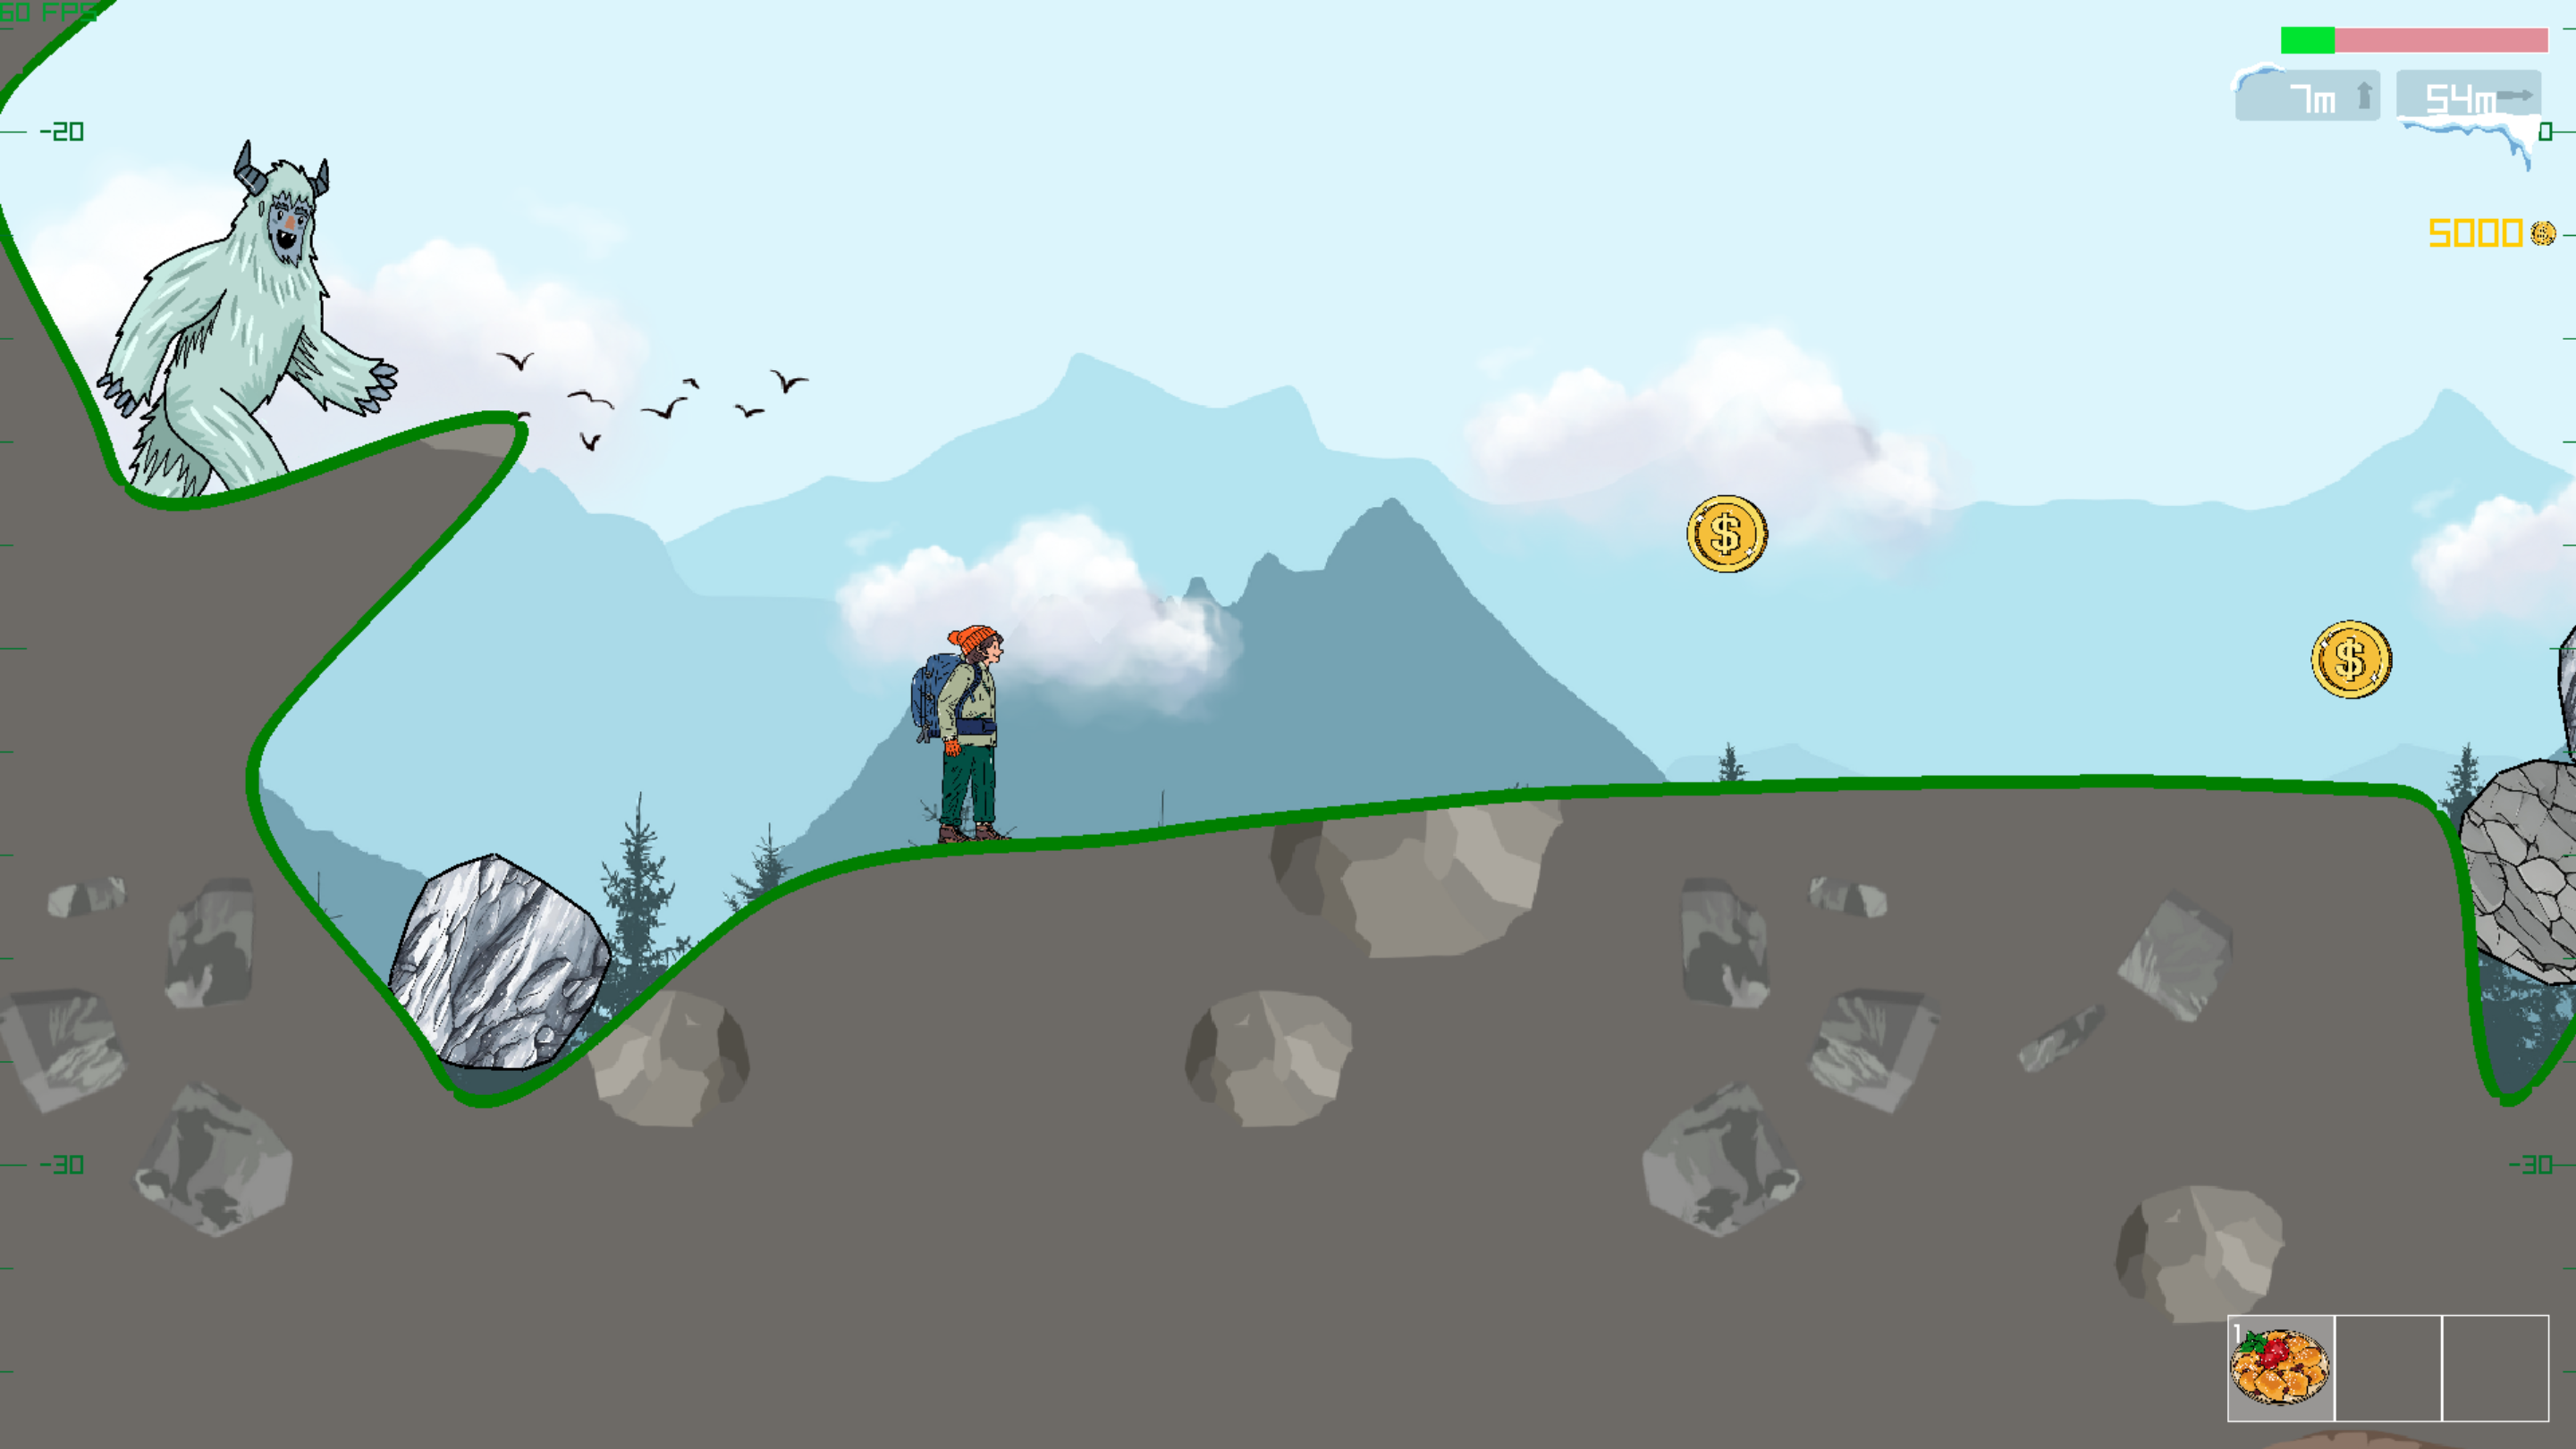
\includegraphics[width=\textwidth]{../figures/Ingame-Picture.png}
            \textbf{Normal Mode}
        \end{minipage}
        \pause
        \begin{minipage}{0.49\textwidth}
            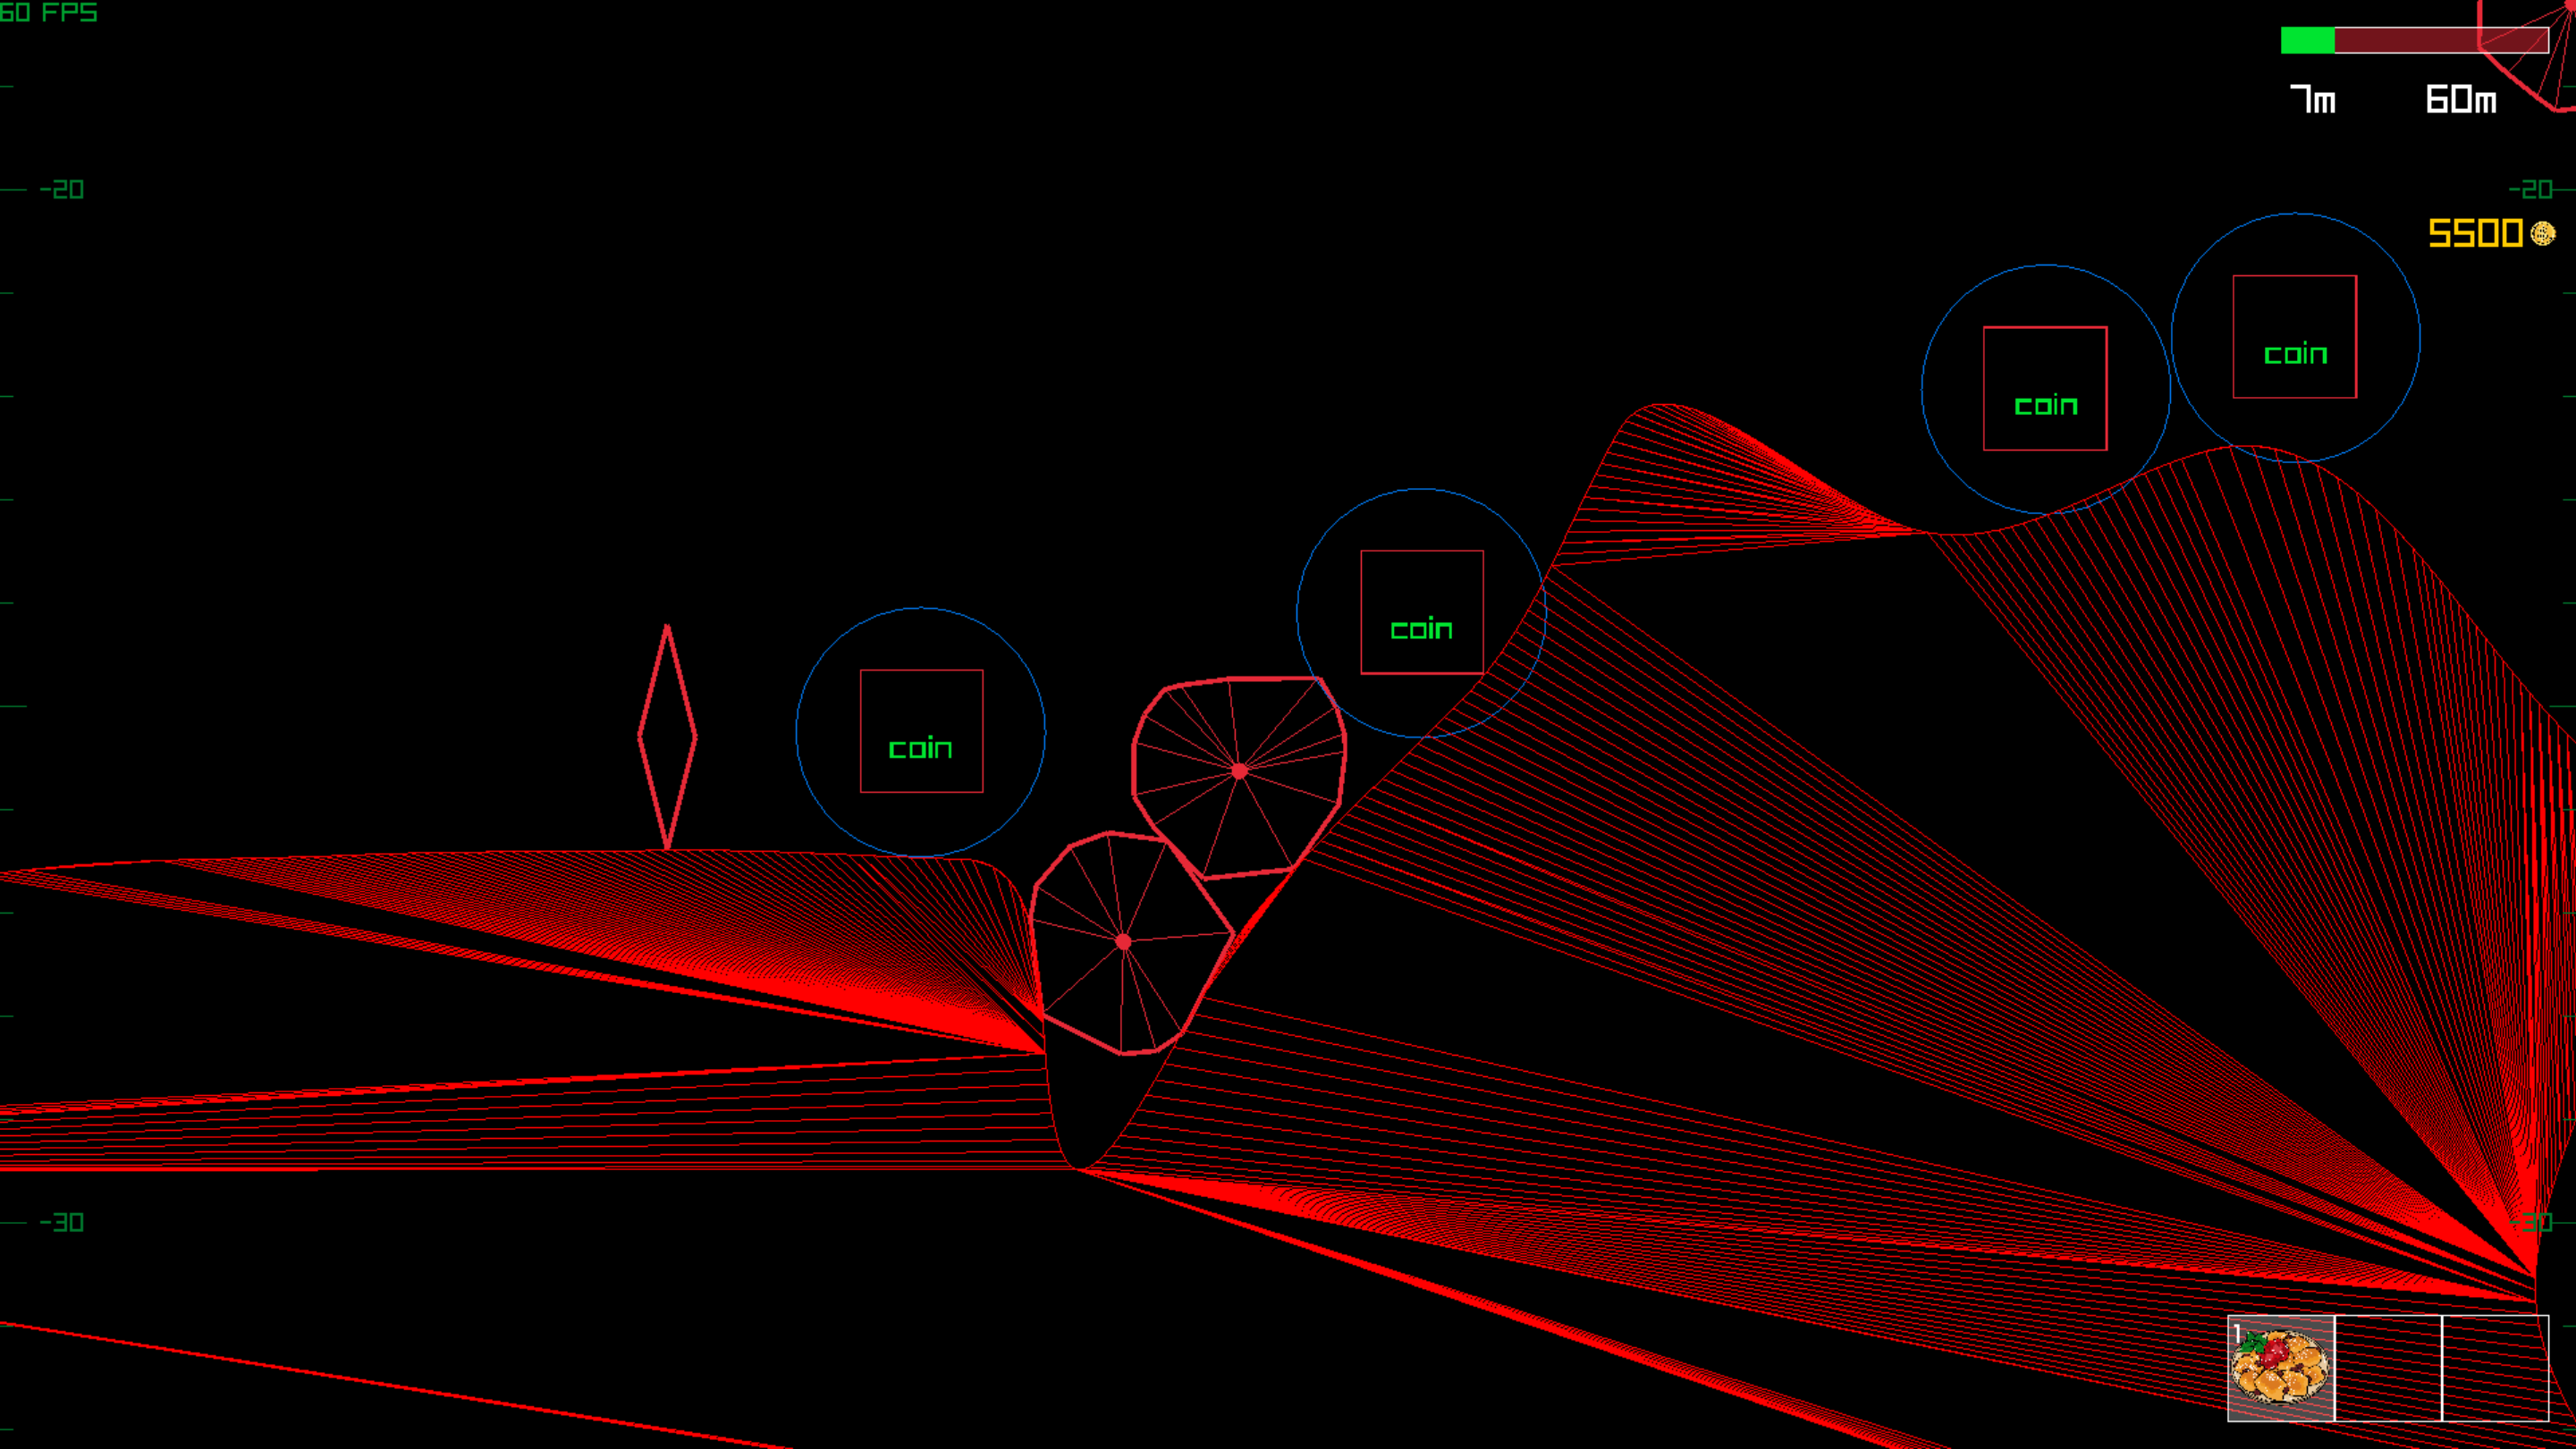
\includegraphics[width=\textwidth]{../figures/Debug-Mode.png}
            \textbf{Debug Mode}
        \end{minipage}
    \end{center}
\end{frame}

